\begin{surferPage}[Kummer-Quartic]{La Quartica di Kummer}
    Nel 1875, Eduard Kummer fu il primo a porre esplicitamente il problema
    di calcolare il massimo numero $\mu(d)$ of singolarit\`a su una superficie di grado
    $d$ . Nel suo caso il grado era $4$ e la superficie \`e detta \emph{quartica}. 
  
  Kummer mostr\`o che $\mu(4)=16$. Dopodich\'e studi\`o le quartiche con $16$
    singolarit\`a in dettaglio.
    Una famiglia particolarmente bella di superfici di questo tipo \`e data da
    \[\bigl(x^2+y^2+z^2-\mu^2\bigr)^2 - \lambda
    \,y_0\,y_1\,y_2\,y_3,\]
    dove $\mu$ \`e un parametro,
    $\lambda = \frac{3\mu^2-1}{3-\mu^2}$;  
     {\small
    $y_0=1-z-\sqrt{2}x$, \  
    $y_1=1-z+\sqrt{2}x$, \ 
    $y_2=1+z+\sqrt{2}y$, \ 
    $y_3=1+z-\sqrt{2}y$}
    sono le facce di un tetraedro regolare
  in modo che la superficie sia simmetrica.
  Non tutte le superfici di questa famiglia hanno esattamente $16$ singolarit\`a reali,
  anche se \`e cos\`i per la maggior parte di esse:
  \begin{center}
    \vspace*{-0.2cm}\hspace*{-0.2cm}
    \begin{tabular}{@{}c@{\,}c@{\,}c@{\,}c@{\,}c@{}}
      \begin{tabular}{@{}c@{}}
        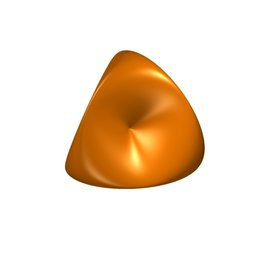
\includegraphics[height=1.4cm]{kummer_0}
      \end{tabular}
      &
      \begin{tabular}{@{}c@{}}
        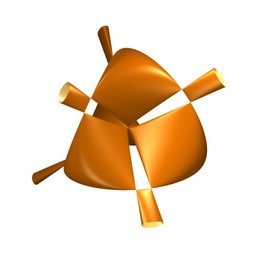
\includegraphics[height=1.4cm]{kummer_1}
      \end{tabular}
      &
      \begin{tabular}{@{}c@{}}
        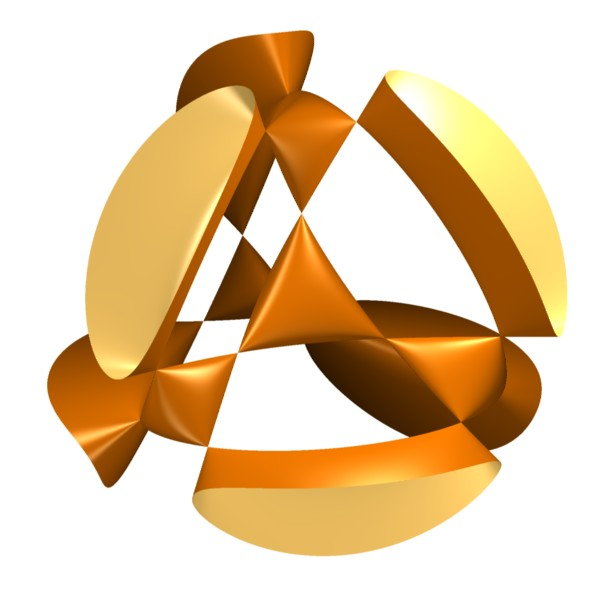
\includegraphics[height=1.4cm]{kummer_2}
      \end{tabular}
      &
      \begin{tabular}{@{}c@{}}
        
\includegraphics[height=1.4cm]{kummer_3}
      \end{tabular}
    \end{tabular}
  \end{center}
  \vspace{-0.2cm}  
   Per certi valori dei parametri, pu\`o capitare che alcune delle singolarit\`a coincidano.
\end{surferPage}
